%%%%%%%%%%%%%%%%%%%%%%%%%%%%%%%%%%%%%%%%%%%%%%%%%%%%%%%%%%%%%%%%%%%%%%%%%%
% Copyright (c) 2011, 2012, ETH Zurich.
% All rights reserved.
%
% This file is distributed under the terms in the attached LICENSE file.
% If you do not find this file, copies can be found by writing to:
% ETH Zurich D-INFK, Universitaetstr. 6, CH-8092 Zurich. Attn: Systems Group.
%%%%%%%%%%%%%%%%%%%%%%%%%%%%%%%%%%%%%%%%%%%%%%%%%%%%%%%%%%%%%%%%%%%%%%%%%%

\documentclass[a4paper,twoside]{report} % for a report (default)

\usepackage{bftn} % You need this
\usepackage{multirow}
\usepackage{listings}
\usepackage{color}

\title{Barrelfish on the Intel Single-chip Cloud Computer}   % title of report
\author{Simon Peter \and Timothy Roscoe \and Andrew Baumann}	% author
\tnnumber{005}  % give the number of the tech report
\tnkey{Single-chip Cloud Computer} % Short title, will appear in footer

% \date{Month Year} % Not needed - will be taken from version history

\begin{document}
\maketitle

%
% Include version history first
%
\begin{versionhistory}
\vhEntry{0.1}{08.02.2010}{SP,TR}{Initial version}
\vhEntry{1.0}{20.07.2010}{SP,TR,AB}{Updates, more detail}
\vhEntry{1.1}{11.08.2010}{SP}{Fill in missing details}
\vhEntry{1.2}{12.08.2010}{TR}{Initial release version}
\vhEntry{1.3}{09.09.2010}{SP,RB}{Corrections to typos and for clarity}
\vhEntry{1.4}{10.05.2012}{SP}{Fake VGA console removed. Physical
  memory layout added.}
\end{versionhistory}

% \intro{Abstract}		% Insert abstract here
% \intro{Acknowledgements}	% Uncomment (if needed) for acknowledgements
% \tableofcontents		% Uncomment (if needed) for final draft
% \listoffigures		% Uncomment (if needed) for final draft
% \listoftables			% Uncomment (if needed) for final draft

\lstset{
  language=C,
  basicstyle=\ttfamily \small,
  flexiblecolumns=false,
  basewidth={0.5em,0.45em},
  boxpos=t,
}

\newcommand{\eclipse}{ECL\textsuperscript{i}PS\textsuperscript{e}\xspace}
\newcommand{\codesize}{\scriptsize}
\newcommand{\note}[1]{[\textcolor{red}{\emph{#1}}]}

%%%%%%%%%%%%%%%%%%%%%%%%%%%%%%%%%%%%%%%%%%%%%%%%%%%%%%%%%%%%%%%%%%%%%%%%
\chapter{Introduction}

This report describes the Barrelfish port to the Intel Single-chip
Cloud Computer \cite{intel:scc:isscc10}.   It serves as a general
repository for information about the SCC platform, and therefore
contains a number of very different kinds of information, for
different audiences.  It should be regarded as an evolving set of
notes, rather than a polished document. 

\begin{itemize}

\item Chapter~\ref{chap:impl} describes the SCC-specific aspects of the
port. This information is of most interest to people trying to
understand the SCC-specific functionality in Barrelfish. 

\item Chapter~\ref{chap:bench} collects various hardware
  microbenchmarks which were used to guide the implementation.  This
  is of interest to those wishing to understand the performance of
  individual operations on the SCC, for example to optimize the 
  Barrelfish implementation. 

\item Chapter~\ref{chap:eval} provides both a quantitative and
  qualitative evaluation of Barrelfish running on the SCC.  This
  summarizes our results of running a limited number of applications
  on Barrelfish using the SCC. 

\item Chapter~\ref{chap:refl} discusses the implications of our early
  experience for future system software on the SCC, and provides some
  thoughts on the suitability of the SCC's hardware for running a
  message-based OS such as Barrelfish.  This deals primarily with how
  well-matched the Barrelfish design is with the hardware features of
  the SCC. 

\item Chapter~\ref{chap:historical} collects information about
  historical features of the port that are not supported anymore.
\end{itemize}

The work described in the current version of this document was carried
out entirely on the ``Copper Ridge'' SCC platform.  
As the Barrelfish project gains more experience with the ``Rocky
Lake'' SCC platform, this document will be updated accordingly. 

We would like
thank Intel Corporation, in particular the SCC team and the Intel
Braunschweig Lab, for their help and early access to the SCC
platform. 


%%%%%%%%%%%%%%%%%%%%%%%%%%%%%%%%%%%%%%%%%%%%%%%%%%%%%%%%%%%%%%%%%%%%%%%%
\chapter{Barrelfish implementation on SCC}\label{chap:impl}

This chapter describes the SCC-specific parts of Barrelfish, and how
they differ from other target architectures.   The SCC port of
Barrelfish is still in its early stages (the version described here is
based on less than 10 person-days of access to early SCC hardware), so
this should be viewed as a preliminary discussion.  

The work was carried out by Simon Peter at the Intel Braunschweig lab
from the 8th to the 12th March 2010, and subsequently from the 26th to
the 30th April 2010. 

\section{CPU driver}

All cores in a Barrelfish system run a CPU driver, which is the only
code which runs in privileged mode on the core.  

The SCC CPU driver is based on the x86-32 port of Barrelfish, and is
identical to it except for not supporting the various address
extensions (PAE, etc.) available on modern 32-bit ia32
machines. Instead, kernel-mode support for multiplexing access to
message passing buffers (MPBs) and configuration registers is
provided.

The SCC CPU driver also supports the x86 UART for debugging output. A
version of the SCC host PC driver\footnote{Available at:
  \url{http://www.dcl.hpi.uni-potsdam.de/research/scc/serial.htm}}
supports a virtual UART for each core on the SCC.

\section{Compilation}

A symbolic target \texttt{scc} has been added to the Barrelfish
makefile. This target carries out two additional steps necessary to
produce a bootable binary image file:

\begin{enumerate}
\item A Barrelfish binary image is compiled from ELF images of the
  kernel and user-space binaries, together with essential bootup
  information (like commandline parameters for those binaries and a
  memory map) from an enhanced GRUB~\cite{grub} \texttt{menu.lst}
  file. This is done using the \texttt{dite} image generation tool,
  written at ETH and included in the \texttt{/tools/dite} directory of
  the Barrelfish source tree. The image is relocated to be loaded at
  address 0xff000.

\item This binary image is converted into Intel 32.obj binary format
  (an Intel-proprietary format) and combined with a 5 byte jump
  vector, to be loaded at address 0xfffffff0, long jumping to
  0x100000, the fixed entry point of the kernel.

\item Another 32.obj file is created, containing only the 5 byte jump
  vector to the same fixed entry point of the kernel.
\end{enumerate}

\section{Boot process: first (bootstrap) core}

The \verb+tools/scc/bootscc.sh+ shell script can be used to boot the
SCC. This script will invoke the following sccKit tools on the host PC
to bootstrap the first SCC core:

\begin{alltt}
  sccReset -g
  sccMerge -m4 -n12 -noimage -lut\_default -force barrelfish48.mt
  sccBoot -g obj
  sccReset -r 0
\end{alltt}

The first \texttt{sccReset} will reset the SCC board into a known
state, in particular all configuration registers.

\texttt{sccMerge} creates memory images for all memory controllers
from the previously created 32.obj files. It will load the boot image
to core 0's memory and load the boot jump vector to all other
cores. The default LUT mappings are created for each core. The file
\texttt{barrelfish48.mt} provided on the commandline is responsible
for this configuration. It is shipped with the Barrelfish source
distribution. \texttt{sccMerge} creates an \texttt{obj} subdirectory
containing the produced memory images. If the directory already
exists, it is removed first.

\texttt{sccBoot} loads the memory images into the memory controllers
from the \texttt{obj} subdirectory.

The second \texttt{sccReset} will release the reset pin of the first
SCC core (core ID 0).

The kernel boot code switches from real mode to protected mode,
activates paging, all caches and the message passing buffers. In
addition to the regular x86-32 startup sequence, it initializes the
in-kernel SCC support code and reads the core ID from the local core
mapping.

The rest of the local boot process is identical to the x86-32 boot
process.

\section{Boot process: subsequent cores}

When told to boot another SCC core with a given core ID, the CPU
driver will modify the booter's LUT mapping to map in the first 16MB
(one LUT entry) of the bootee at a known fixed address, known not to
contain useful memory of the booter.

The booter will then ELF load a copy of the CPU driver to address
0x10000 and append copies of the ELF binaries of the CPU driver, the
monitor, init, and mem\_serv. These programs are needed to bring up
the bootee core. A special configuration region at address 0xff00 is
also written to inform the bootee that it is an application kernel,
the address of the inter-monitor CC-UMP message passing region in
shared RAM, the location of the binary copies, as well as the
notification channel ID used for that channel. CC-UMP and notification
channels are described in Section~\ref{sec:interconnect}.  Then, the
reset pin of the bootee is released via configuration registers.

\section{Physical address space}

The SCC allows the physical address space of each core to be
configured using the 256-entry Lookup Table~\cite{rockcreek_eas}
(LUT).  In normal operation, we use the default LUT memory map, as is
used by Intel for the Linux OS, and amend it for extra physical memory
if available. The memory map is described in the
\verb+hake/menu.lst.scc+ file, and inserted into the boot image by the
\verb+dite+ tool, where the kernel can find it.

\begin{center}
\begin{tabular}{lll}
Area & start & end\\
\hline
Private DDR3 RAM & 0 & 0x28ffffff \\
Remote boot LUT & 0x29000000 & 0x29ffffff \\
\emph{Unused} & 0x2a000000 & 0x7fffffff \\
Shared DDR3 RAM & 0x80000000 & 0xbfffffff \\
On-tile MPBs & 0xc0000000 & 0xd7ffffff \\
Local on-tile MPB & 0xd8000000 & 0xd8ffffff \\
\emph{Unused} & 0xd9000000 & 0xdfffffff \\
Configuration registers & 0xe0000000 & 0xf7ffffff \\
Local configuration regs & 0xf8000000 & 0xf8ffffff \\
eMAC access & 0xf9000000 & 0xf9ffffff \\
TCP/IP traffic (unused) & 0xfa000000 & 0xfaffffff \\
RPC (unused) & 0xfb000000 & 0xfbffffff \\
SATA (unused) & 0xfc000000 & 0xfcffffff \\
\emph{Unused} & 0xfd000000 & 0xfeffffff \\
Private DDR3 RAM & 0xff000000 & 0xffffffff \\
\end{tabular}
\end{center}

\section{Virtual address space}

The available virtual address space on a core is split into 2GB
user-space access (addresses 0x0 -- 0x7fffffff) and 2GB for
kernel-only access (addresses 0x80000000 -- 0xffffffff).

The kernel-only space maps directly to physical address 0x0 until
0x3fffffff, allowing access to all of private RAM with the default LUT
mapping. This resembles mappings used in single address space
operating systems and provides better performance when handling kernel
objects than can be provided with classical operating systems, like
Linux. Kernel objects can point to other objects directly and the
mapping is identical across all cores. Also, physical addresses can be
calculated simply by subtracting an offset, instead of via complicated
mappings.

Space is reserved at the top of this range to map all MPBs and all
configuration registers, as well as the local APIC and one remappable
4K page to map in a foreign core's private RAM, used for booting that
core.  The rest of kernel virtual address space is unused. This
implies that kernel objects can only be created in the lower 2GB of
physical memory (ie. in private RAM), which is sufficient in
Barrelfish, as kernel objects are never shared between cores.

The user-space address range can be arbitrarily mapped to physical
addresses.

\section{Memory allocation}

A memory allocation server (\texttt{mem\_serv}) is spawned for every
on-line core in the system.

Available shared RAM is equi-partitioned into 48 regions. Remaining
shared RAM not fitting this partition is thrown away and is not
usable. The reason for this is that the memory allocators are not able
to handle allocation from unaligned memory regions and sizes that are
not a power of two.

The server gets given capabilities for all of the private RAM of the
local core and \textbf{all of shared RAM}. This is necessary so that
allocation of shared mappings is possible from every core's region
without having to contact a designated memory allocator for this
region of RAM, a feature not yet implemented.

As shared RAM is handled identical to private RAM, the kernel is
responsible for clearing a newly allocated page of memory from
previous usage before allowing it to be mapped into the allocator's
address space. As shared RAM resides outside the lower 2GB of physical
address space, the kernel is incapable of accessing that RAM in order
to clear it. For SCC, we have modified the kernel to instead neglect
clearing the page, at the expense of protection when memory is reused
from other address spaces.

This issue is fixable however, either by reserving another remappable
address range inside the kernel that can be used to map and clear the
page before allowing the user to map it, at an expense of
performance. Another way to fix it is to introduce a special memory
allocator for shared RAM that would map and clear allocated RAM first
into its own address space before granting it to the requesting
address space.

Per-core memory servers are necessary on SCC. Memory servers do not
currently support allocation from multiple private RAM regions with
overlapping address regions.

\section{Interconnect driver}\label{sec:interconnect}

In Barrelfish, an interconnect driver is the lowest-level part of a
particular messaging mechanism. The inter-core interconnect driver for
the SCC is based on the cache-coherent user-level message passing
(CC-UMP) driver used by Barrelfish on x86 systems. With some
modifications this mechanism reliably transports cache-line-sized
messages through non-coherent shared memory on SCC.

The modifications are:
\begin{itemize}
\item The size of a cache-line, and thus message, is 32 bytes.

\item Memory for both the send and receive message channel is
  allocated in the core's region of shared RAM that is initiating a
  bind to another core, using the NUMA allocation features of
  Barrelfish. These are currently not thread-safe and thus the
  interconnect driver initialisation phase is currently not
  thread-safe.

\item Memory for the message channel is mapped as cacheable, message
  passing buffer type, enabling the use of the write-combining buffer
  for faster memory writes. For this, the implementation of the
  virtual memory manager inside \texttt{libbarrelfish} had to be
  extended to support the architecture-specific mapping flags.
\end{itemize}

While CC-UMP was originally optimized for cache-coherent transports, these
optimizations do not hurt performance on SCC and we are not aware of other
SCC-specific optimizations that CC-UMP does not already employ.

However, the polling approach used by CC-UMP on Barrelfish to detect incoming
messages is inappropriate on the SCC, since each poll of a message-passing
channel requires a \texttt{CL1INVMB} operation followed by a load from DDR3
memory.

Consequently, an additional SCC notification driver (named
\texttt{rck\_notify}) was implemented which augments the CC-UMP driver
with notification support. For this, support for pluggable
notification drivers was added to CC-UMP.

The notification driver uses the on-tile MPB for efficiently
communicating the identifiers of active message channels, and
an inter-core interrupt as the notification mechanism. It is implemented
mostly within the CPU driver on each core, as follows: \note{AB: Diagram?}

\begin{itemize}
\item A ring-buffer of IDs of those channels containing unread payload
  is held in the receiver's MPB. The buffer is written only by senders and
  read only by the receiver. However, there are two read-shared
  cache lines before the buffer, holding the current write and current
  read position, respectively.
\item A buffer entry spans a cache-line (32 bytes). Currently, only a
  16-bit channel ID is written to that cache-line, limiting the number
  of distinct notifiable channels to 65,536. The rest of the space in
  unused. Using a cache-line per ID allows a sender to write new
  channel IDs to the buffer without having to read the cacheline for
  already existing IDs first.
\item A new capability type is used on the sender side, holding the
  core ID and channel ID of the receiver core of the
  notification. When invoked, the sender's CPU driver:
  \begin{enumerate}
   \item Acquires the test-and-set lock for the receiving core
   \item Reads the current write position from the receiver's MPB
   \item Writes the channel ID into the next slot in the reciever's MPB
   \item Updates the current write position in the receiver's MPB
   \item Reads the receiver's interrupt status
   \item If no inter-core interrupt is pending, writes the status word
         with the interrupt set to trigger a remote interrupt
   \item Clears the test-and-set lock for the receiving core
  \end{enumerate}
\item On the receiver, a regular LMP endpoint capability is registered
  in a special notification table inside the CPU driver. This table maps
  channel IDs to local LMP endpoints that will be signalled on notification.
  When the receiver core is interrupted, it looks up all pending channel IDs
  present in the MPB ring-buffer, and dispatches an empty message on the
  registered endpoint in the table. If no endpoint is registered, an error
  is signalled.
\item In user-space, the notification driver triggers the waitset used
  to wait on incoming messages for the corresponding message channel,
  activating the receive message handler in the generated stubs, which
  are described in the following section.
\end{itemize}

In case of the receiver ring buffer being full when the sender tries
to write a new channel ID, the sender aborts the process and returns
with an error code to the sending user-space application, indicating a
failed notification. The user-space application should try to notify
the receiver again at a later point in time (currently unimplemented
as we did not reach this case during our benchmarks). Rolling back the
message send is not easily possible, as the receiver might have been
actively polling for and already reading it.

Allocation of new channel IDs is managed by the monitor of the
receiving core as part of the bind process. The CPU driver does not
allocate IDs.

There are many design alternatives for an SCC interconnect driver, and
the above should be regarded as only one point in the space.  At first
sight, it may seem odd to use main memory (rather than the on-tile
MPB) for passing message payloads, and to require a trap to the kernel
to send a message notification.

This design is motivated by the need to support many message channels
in Barrelfish and, furthermore, more than one application running on a
core.  The SCC's message-passing functionality does not appear to have
been designed with this use-case in mind.
We discuss this issue further in Chapter~\ref{chap:refl}. 

We considered two further design alternatives: \emph{notification
  trees} and \emph{payload in MPB}. The former we have implemented and
benchmarked, but it turned out to have worse performance than the ring
buffer implementation presented above.

Notification trees use the same notification scheme as ring buffers,
but employ a bitmap of channel IDs, represented as a two-level tree in
the receiver's MPB. One bit for every distinct channel that can be
notified. Tree nodes are of the size of one cache-line (256 bits). The
tree's layout in the ring buffer is such that the root node occupies
the first cache-line. All other nodes are leaves and are stored in
left-to-right order after the root node. There are 255 leaves which
contain a bit for each notifiable channel, yielding 65,280 notifiable
channels. A bit set in the root node indicates that the corresponding
leave contains set bits and should be scanned when the tree is
traversed. In this scheme, sending a notification can never fail: A
bit can either be set or is already set, in which case no further
notifications need to be sent for the respective channel ID.

Sending a notification for a given channel ID in this design requires
the sender to:

\begin{enumerate}
\item Acquire the test-and-set lock for the receiving core
\item Read the root node from the receiver's MPB
\item Set the bit for the corresponding leaf node of the channel ID
  in the root node
\item Write the root node to the receiver's MPB
\item Read the leaf node from the receiver's MPB
\item Set the bit for the corresponding channel ID in the leaf node
\item Write the leaf node to the receiver's MPB
   \item Read the receiver's interrupt status
   \item If no inter-core interrupt is pending, write the status word
     with the interrupt set to trigger a remote interrupt
\item Clear the test-and-set lock for the receiving core
\end{enumerate}

This mechanism requires 2 full cache-line reads and 2 full cache-line
writes from/to the receiver's MPB and 2 bit operations as opposed to
only two 32-bit reads and 2 full cache-line writes in the ring buffer
scheme. We originally proposed notification trees, assuming the cost
to access remote MPBs would be an order of magnitude lower, as well as
cheaper bit operations on full cache-lines. After implementing and
benchmarking this scheme, it turned out not to be the case. We assume
the slow bit operations to be due to the size of the operands. Holding
a full cache-line would require 8 integer registers on the Pentium.
With only 7 present, we always have to go to memory in order to
execute a bit-scan, an expensive operation, especially when the cache
does not allocate on a write miss.

The final design we devised is ``payload in MPB''. In this scheme,
instead of notifying the receiver of a message in shared RAM, the
message payload itself is written to the MPB, obliviating the need for
shared RAM. The main drawback of this scheme is that it requires quite
complicated book-keeping, as messages are variable size and might not
fit into the rather small 8KB receive buffer.

It also complicates managing quality of service, as multiple
applications now compete for the same receiver MPB. This forbids
receiving applications the use of the payload inside the MPB directly,
as the MPB has to be freed up as quickly as possible to allow other
competing applications to make progress. This requires copying the
message out of the MPB into private RAM of the receiver, which is
again a costly operation, especially as caches do not allocate on a
write miss. We elaborate more on this issue in
Chapter~\ref{chap:refl}.

\section{Message passing stubs}

In Barrelfish, message-passing stubs are the next layer of functionality
above the interconnect driver, and implement typed variably-sized messages
over various interconnects. They are generated by our stub-generation tool,
named \emph{Flounder}.

The Flounder backend for SCC message passing is derived from, and shares much
code with, the backend for CC-UMP. The important differences are:

\begin{itemize}
\item The generated stubs are configured for a cache-line size of 32 bytes,
  and thus the message-fragments used to transmit message payload are never
  more than 32-bytes in size.
\item The binding logic allocates and initialises the SCC notification
  endpoints, and transmits their capabilities to the receiver.
\item The code to send messages is modified to emit a notification either at
  the end of a complete (application-level) message, or when the message
  channel ring buffer is full and the sender needs to block. In this way,
  needless notifications (for fragments of a high-level message) are avoided.
\item The receive side never polls for incoming messages. When no more messages
  are present in the channel, it instead blocks on a waitset that will be
  signalled when an inter-core notification arrives.
\end{itemize}

\section{Bulk transfer}

Bulk transfer shared memory is mapped the same way as CC-UMP
memory on SCC (cacheable, MPB).  

As shared memory is directly manipulated by the application for a bulk
transfer region, the bulk\_prepare() function for SCC touches a random
cacheline that is not of the bulk transfer region. This forces the
write combine buffer to flush the last written cacheline out to
memory (see Section 1.4.5 of~\cite{rockcreek_core_eas}). This needs
to be done, as an application may have written an incomplete cacheline
to the transfer area, to force that line out to memory before sending.

%%%%%%%%%%%%%%%%%%%%%%%%%%%%%%%%%%%%%%%%%%%%%%%%%%%%%%%%%%%%%%%%%%%%%%%%
\chapter{Hardware measurements}\label{chap:bench}

Cost of assorted local operations: 

\begin{center}
\begin{tabular}{rl}
operation & cycles \\
\hline \\
NOP system call & 200 \\
RDTSC instruction & 14 \\
XCHG instruction & 35 \\
LOCK CMPXCHG instruction & 39 \\
LOCK DEC instruction & 36 \\
clear memory & 3 \\
NOP instruction & 2 \\
CL1INVMB & 1 \\
\end{tabular}
\end{center}

Cost in cycles to write a complete 32-byte cache line (8 DWORD writes)
to an on-tile MPB from a core on tile 0:

\begin{center}
\begin{tabular}{cc|cccccc}
&  &\multicolumn{6}{c}{\textit{target tile x-coordinate}} \\
 &   & 0   & 1   & 2   & 3   & 4   & 5 \\ \hline 
\multirow{4}{*}{\textit{y}} & 0 & 39  & 84  & 89  & 90  & 95  & 101 \\
 & 1 & 84  & 89  & 89  & 95  & 101 & 108 \\
 & 2 & 89  & 89  & 95 & 101 & 107 & 113 \\
 & 3 & 89  & 95  & 101 & 108 & 113 & 119 \\
\end{tabular}
\end{center}

Cost to read a single DWORD from on-tile MPBs from tile 0 (this will
pull the cache line into local L1 on tile 0):

\begin{center}
\begin{tabular}{cc|cccccc}
&  &\multicolumn{6}{c}{\textit{source tile x-coordinate}} \\
 &   & 0   & 1   & 2   & 3   & 4   & 5 \\ \hline 
\multirow{4}{*}{\textit{y}} & 0 & 20  & 63  & 69  & 72  & 78  & 84 \\
 & 1 & 63  & 69  & 72  & 78  & 84  & 90 \\
 & 2 & 69  & 72  & 78  & 84  & 90  & 96 \\
 & 3 & 72  & 78  & 84  & 90  & 96  & 102 \\
\end{tabular}
\end{center}

\section{Memory map and shared memory areas}

In this benchmark, a user-space application reads/writes repeatedly
from/to shared memory, using different mapping configurations. Core 0
executed this benchmark. All numbers presented are in machine cycles.

\begin{center}
\begin{tabular}{cccl}
\hspace{3em} & Memory controller & average & total for 1,000,000 iterations \\
\hline \\
\multicolumn{4}{l}{DWORD from shared RAM (uncacheable):} \\
\\
 & 0 & 97  & 97,338,585 \\
 & 1 & 121 & 121,492,066 \\
 & 2 & 105 & 105,348,809 \\
 & 3 & 134 & 133,690,789 \\
\\
\multicolumn{4}{l}{Cacheline to shared RAM (uncacheable):} \\
\\
 & 0 & 779 & 778,680,899 \\
 & 1 & 972 & 971,920,810 \\
 & 2 & 843 & 842,761,220 \\
 & 3 & 1069 & 1,069,474,168 \\
\\
\multicolumn{4}{l}{Cacheline to shared RAM (MPB):} \\
\\
 & 0 & 122 & 121,504,321 \\
 & 1 & 146 & 146,014,496 \\
 & 2 & 134 & 133,697,675 \\
 & 3 & 158 & 157,781,513 \\
\end{tabular}
\end{center}

\section{Thread Switch Time}

In this benchmark two threads are yielding between each  other in a
ping-pong like benchmark. Therefore, Barrelfish's
thread\_yield\_dispatcher function is used. This function donates the
callers time-slice to the dispatcher pointed to by the argument to this
function.

A call to this function requires an endpoint capability to the
partner, which needs to be exchanged between the threads at
startup. One of the dispatchers acts as a server, calling export to
offer the service to the nameserver, the other one as a client calling
the bind function.

The waitloops are broken as soon as both partners have the required
endpoint capabilities set up. When looking at the numbers given in
this benchmark, it is important to keep in mind that the domains might
run some event processing code on scheduling.

The decision to include those numbers in the measurements is on
purpose for this analysis.

The number of cycles given is from one thread to the partner and back
to the original thread and therefore needs to be divided by two to get
an approximation for the actual thread switch time.

\begin{center}
\begin{tabular}{rl}
thread & cycles \\
\hline \\
server & 6732.79\\
client & 6636.08\\
\end{tabular}
\end{center}


%%%%%%%%%%%%%%%%%%%%%%%%%%%%%%%%%%%%%%%%%%%%%%%%%%%%%%%%%%%%%%%%%%%%%%%%
\chapter{Evaluation of the implementation}\label{chap:eval}

This chapter describes the effort required to bring up Barrelfish on
the SCC, together with early micro- and application benchmark
results. 

\section{Development effort}

Bringing up Barrelfish on the SCC first required a 32-bit ia32 port,
since up to that point we had only targetted 64-bit Intel Archtecture
platforms.  This port was carried out in advance by Simon using a
mixture of real hardware and QEMU configured to emulate a Pentium
processor, and substantially reduced the time required on actual SCC
hardware. 

The process was also helped by Orion Hodson's ARM port, and Richard
Black's Beehive port, which threw up many 64-bit dependencies at an
early stage.  In the event, most of these issues were resolved well
before the SCC port started. 

Lines of code, using David Wheeler's SLOCCount:

\begin{itemize}
% \item Using SLOCcount on only the x86-32 specific code yields 6108
%   lines of C code and 130 lines of assembly code (not counting
%   imported code, like libc or libm). Out of this, 70\% is kernel
%   code.

\item As of August 11, 2010, the x86-32 specific code yields 8705
  lines of C code and 410 lines of assembly code (not counting
  imported code, like libc or libm). Out of this, 6011 lines (69\%) is
  kernel (CPU driver) code.

\item In addition to the x86-32 specific code, 2235 lines of
  SCC-specific C code and 130 lines of assembly code were written, 391 
  lines (17\%) of these being CPU driver. This count does not include
  the sections of x86-32 specific code that have workarounds for SCC
  using \#ifdef constructs.
\end{itemize}

By and large, the bringup for SCC was straightforward:


\begin{itemize}
\item Porting back from x86-64 using a memory-window
  based model for kernel state allowed us to keep the programming
  model and general address space layout.  One minor issues was the
  requirement to initialize shared RAM from
  user-space.  This makes it unsafe to allow regular user-space
  applications access to untyped memory, as they could snoop its
  previous content without erasing the memory.

\item At the time of the x86-32 port, most arch-generic Barrelfish
  code was still mostly x86-64-specific and so time was spent on
  separating out arch-specific quirks from otherwise generic code and
  clean-up. 

\item The message passing transport was designed within one
  day. However, it turned out it was not as efficient as expected, due
  to our (overly optimistic) assumptions about memory access latencies.

\item Overall, the work took about 2 person-months.
\end{itemize}

At time of writing, we believe the major performance issues with our
code are due to the SCC L2 caches' non-allocate-on-write policy. Our
code is not optimized for this behavior and shows major
inefficiencies, in particular on function call boundaries immediately after
kernel crossings.

% \section{Measurements}\label{sec:measurements}

% %    * Breakdown of IPI pingpong benchmark (cores 0 \& 1): 16722
% %     * Sender: Into kernel, up to rck\_send\_notification(): 687 cycles
% %     * Sender: Time taken for rck\_send\_notification(): 605 cycles
% %     * Sender: Upon receipt of message from peer: 7987 cycles

% %    * cores 0 \& 2: 17372
% %     * Sender: Into kernel, up to rck\_send\_notification(): 687 cycles
% %     * Sender: Time taken for rck\_send\_notification(): 794 cycles
% %     * Sender: Upon receipt of message from peer: 8224 cycles

% %    * cores 0 \& 10: 17794
% %     * Sender: Into kernel, up to rck\_send\_notification(): 688 cycles
% %     * Sender: Time taken for rck\_send\_notification(): 927 cycles
% %     * Sender: Upon receipt of message from peer: 8371 cycles

% %    * As you can see, latency goes up the further the cores are away.

\section{Microbenchmark: Notification via MPB}\label{sec:mpb_bench}

We implemented a ping-pong notification experiment to evaluate the
cost for OS-level notification delivery via message passing buffers
(MPBs). MPB notifications are used in Barrelfish to notify a
user-space program on another core of message payload arrival on a
CC-UMP channel and are thus performance critical.

The experiment entails two peer cores sending notifications back and
forth. Based on their roles, we call these two cores \emph{initiator}
and \emph{collaborator}, respectively. The experiment is driven by a
user-space program on the initiator. After setup, one iteration of the
experiment is carried out in several steps. The experiment as depicted
by Figure~\ref{fig:mpbbench} is symmetric, thus we only describe the
steps carried out and observed by the initiator:

\begin{enumerate}
\item The initiator's monitor calls a special system call to send a
  message directly to the collaborator and control is transfered to the
  initiator's CPU driver.

\item The initiator's CPU driver writes the message into the collaborator's
  MPB and sets the corresponding configuration registers of the collaborator
  to raise its hardware INTR line.

\item The collaborator receives the message and replies, by carrying out
  steps 4, 1 and 2 in that order \note{AB: unclear}.

\item The initiator's CPU driver traps upon receiving the interrupt,
  determines the cause for the trap, reads the message from its MPB
  and transfers control back to its monitor, which records the time
  taken for all 4 steps.
\end{enumerate}

\begin{figure}
  \centering
  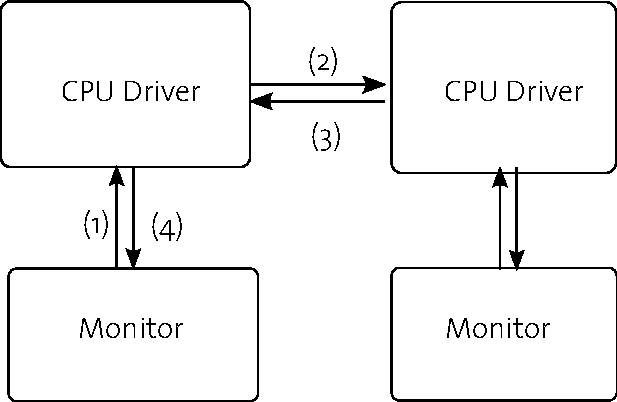
\includegraphics[width=6cm]{figures/exp1}
  \caption{MPB ping-pong experiment setup}
  \label{fig:mpbbench}
\end{figure}

% \note{AB: Need to describe clock speed config somehwere}

We carried out this benchmark between core 0 and all other cores
inside the system, measuring the round-trip latency for an MPB
message containing one cacheline, and halved the result to extrapolate
the one-way latency. Figure~\ref{fig:mpbresults1} shows the result, as
well as a break-down into interesting steps of the experiment.

\begin{figure}
  \centering
  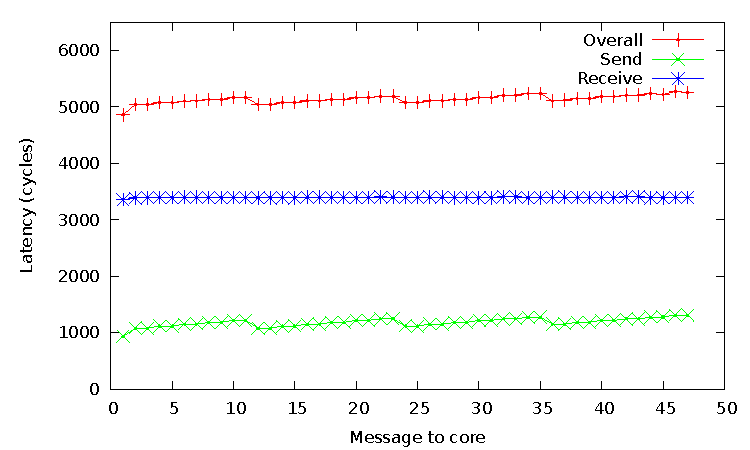
\includegraphics[width=\textwidth]{plots/mpbbench/mpbbench_oneway.pdf}
  \caption{MPB one-way messaging latency from core 0
    (\emph{Overall}). \emph{Send} shows cumulative latency in steps 1
    and 2. \emph{Receive} shows latency of step 4.}
  \label{fig:mpbresults1}
\end{figure}

% Absolute numbers for IPI benchmark with optimization \texttt{-O3}, no
% interrupts, array: \note{Please clarify what this benchmark is what
%   ``array'' means.  Also, assume these are cycles as well?}

% \begin{center}
% \begin{tabular}{ p{0.2\textwidth}|p{0.3\textwidth}}
% op & cycles \\
% \hline \\
% send: & 800 (includes user-space): \\
% receive: & 2596 (includes user-space): \\
% round-trip with both monitors: &  7026 \\
% extrapolated one-way latency for short message: & 3513\\
% \end{tabular}
% \end{center}

\section{Microbenchmark: Inter-processor interrupt (IPIs) latency}

We modify the message latency ping-pong experiment described in
Section~\ref{sec:mpb_bench} to approximate the cost for hardware-level
inter-processor interrupt delivery. IPIs are used in Barrelfish to
notify another core of message arrival and are thus performance
critical.

The core roles are kept and the numbers presented are still for two
cores on the same tile. After setup, one iteration of the experiment
is carried out in 5 steps, as depicted by Figure~\ref{fig:ipibench}:

\begin{enumerate}
\item The initiator's monitor calls a special system call to send a
  message directly to the collaborator and control is transfered to the
  initiator's CPU driver.

\item The initiator's CPU driver writes the message into the collaborator's
  MPB and sets the corresponding configuration registers of the collaborator
  to raise its hardware INTR line.

\item The collaborator's CPU driver traps upon receiving the interrupt,
  determines the cause for the trap, reads the message from its MPB
  and immediately replies with another message to the initiator, using
  the mechanism of step 2, upon which the initiator's CPU driver
  traps.

\item Upon determining the trap cause, the initiator's CPU driver
  reads the message from its MPB.

\item The initiator's CPU driver transfers control back to its
  monitor, which records the time taken for all 4 steps.
\end{enumerate}

% \note{AB: This is more than an IPI!}

\begin{figure}
  \centering
  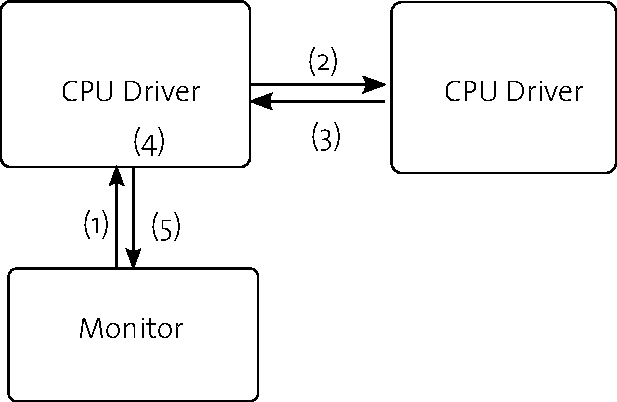
\includegraphics[width=6cm]{figures/exp2}
  \caption{IPI ping-pong experiment setup}
  \label{fig:ipibench}
\end{figure}

In this version of the experiment, which ran over 100,000 iterations,
eliminating the first 10\% of values, the average time for an IPI
round-trip is 8746 cycles. Table~\ref{tab:ipiresults} presents a
break-down of the measured costs. The measured average latency for
step $i$ is denoted as $\lambda_i$. We did not collect measurements
for all steps individually and some measurements are only made for
steps in combination.

We can then approximate the latency $\lambda_{IPI}$ involved to
deliver the IPI, including the time to execute the trap, by
$\lambda_{IPI} = \frac{\lambda_3 - (\lambda_2 + \lambda_4)}{2}$, the
total time spent inside the peer kernel, minus the time to send and
receive an IPI inside the local kernel, divided by two to yield the
time needed for only one trap (we are in a ping-pong loop).

Note that this is an optimistic approximation. As the local side
includes user-code to drive the benchmark, the measured latencies
inside the local kernel might be too large, due to missing cache lines
caused by executing user code. As this cost does not occur on the peer
kernel, where only kernel code is executed, the real cost for an IPI
might be higher. Furthermore, we only measured the cost for two
kernels on the same tile. The cost to deliver an IPI between cores of
far away tiles might be slightly higher.

\begin{table}
  \centering
  \begin{tabular}{p{0.2\textwidth}|p{0.2\textwidth}}
    op & cycles \\
    \hline \\
    $\sum_{i=1..5}{\lambda_i}$ & 8746 \\
    $\lambda_1 + \lambda_2$ & 1135 \\
    $\lambda_4 + \lambda_5$ & 3864 \\
    $\lambda_2$ & 684 \\
    $\lambda_3$ & 3662 \\
    $\lambda_4$ & 1754 \\
    $\lambda_{IPI}$ & \textbf{612} \\
  \end{tabular}
  \caption{Measured and extrapolated IPI benchmark latencies}
  \label{tab:ipiresults}
\end{table}

We consider a latency of at least 612 cycles to deliver an IPI very
high for it to be useful as a signaling primitive for the majority of
message sends in a message-passing system like Barrelfish.

\section{Application-level benchmarks}

The only other software environment presently available on SCC uses a
separate instance of the Linux kernel on each core. Above this runs
RCCE~\cite{intel:rcce}, a library for light-weight, efficient
communication that has been co-designed with SCC as a research vehicle
for message-passing API design on non-cache-coherent many-core chips,
and as such is highly optimized for this platform. RCCE runs in
user-mode with raw access to the MPBs, providing basic point-to-point
message passing functionality as well as a set of higher-level
primitives, such as barriers and a reduce operation, akin to those
found in MPI~\cite{mpi}.

We implemented a substrate supporting the RCCE message-passing
interface using Barrelfish stubs and interconnect drivers for
messaging, and thus can securely support multiple applications. We
evaluated the NASA benchmarks shipped with RCCE to compare the
performance achieved on Barrelfish to a system running 48 instances of
Linux, as used at Intel.

Figures \ref{fig:appresults_total} and \ref{fig:appresults_speedup}
show the result of this comparison. We can see that at the application
level, when a single application is run, Barrelfish does show only
slightly lower performance than 48 Linux instances. We attribute this
to the early version of our port. There is no reason why Barrelfish
should not have identical performance to 48 instances of Linux when
only a single application is run. We furthermore expect Barrelfish to
have better performance than the Linux setup when multiple
applications need to be scheduled on the SCC.

\begin{figure}
  \centering
  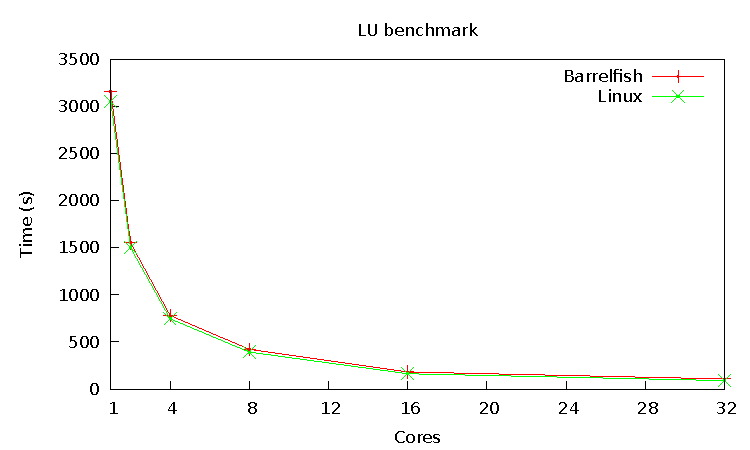
\includegraphics[width=.5\textwidth]{plots/rcce_bench/rcce_lu.pdf}%
  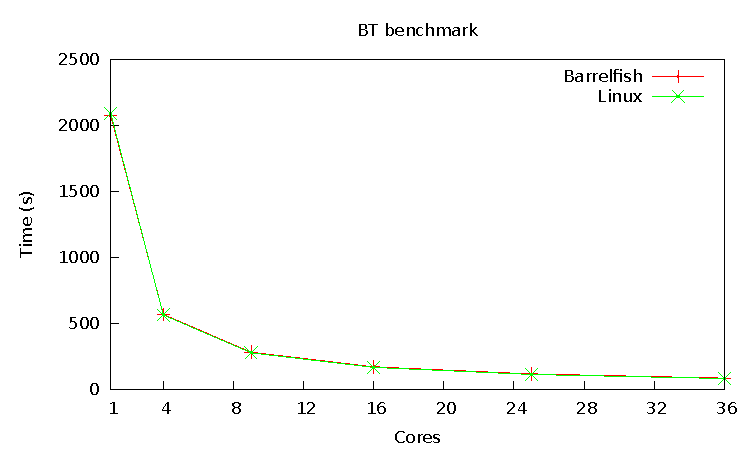
\includegraphics[width=.5\textwidth]{plots/rcce_bench/rcce_bt.pdf}
  \caption{RCCE benchmark absolute performance comparison}
  \label{fig:appresults_total}
\end{figure}

\begin{figure}
  \centering
  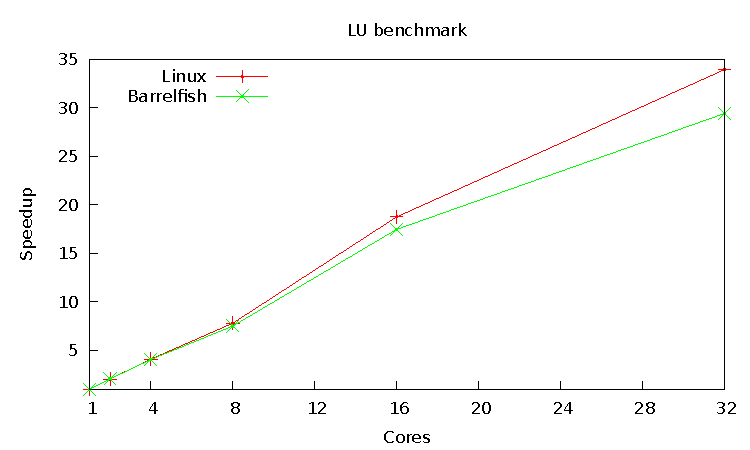
\includegraphics[width=.5\textwidth]{plots/rcce_bench/rcce_lu_speedup.pdf}%
  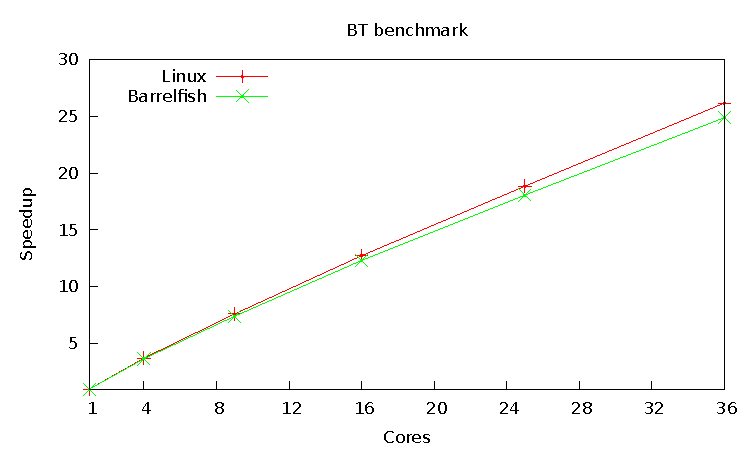
\includegraphics[width=.5\textwidth]{plots/rcce_bench/rcce_bt_speedup.pdf}
  \caption{RCCE benchmark speedup comparison}
  \label{fig:appresults_speedup}
\end{figure}

%%%%%%%%%%%%%%%%%%%%%%%%%%%%%%%%%%%%%%%%%%%%%%%%%%%%%%%%%%%%%%%%%%%%%%%%
\chapter{Reflections on SCC as a platform}\label{chap:refl}

This chapter contains a set of reflections on the challenges of
implementing Barrelfish on SCC hardware.  It should be regarded as a
snapshot of our current thinking, rather than a definite set of
conclusions.  Indeed, as our understanding of how to effectively
exploit SCC as a platform evolves, we expect some of these views to
change.  We would warmly welcome any feedback or suggestions with
regard to this points.  

\section{Build environment}

SCC is a straightforward platform for us to build Barrelfish for -- we
already cross-compile for 32- and 64-bit Intel Architecture machines,
and the P54C is fully supported by gcc. 

Two features of the SCC development environment could be improved (or
were during the porting process): 

\begin{itemize}
\item The tools provided for board setup, initialization, console,
  etc. were all GUI-based, making it impossible to script commonly
  used processes.  All the boot tools used for Barrelfish at ETHZ and
  MSR are command-line based, and fully automated (for example, our
  regression tools start by powering on the machine and turn the
  hardware off when done) and we use build-and-boot scripts
  extensively.  The bringup process would have been considerably
  faster with CLI tools for board control.

  Many of these tools exist (partly as a result of our feedback), but
  it would be helpful if the command-line interface was regarded as a
  first-class requirement. 

\item A proper console driver (a low-level, bidirectional character
  channel between the HCPC would have been very useful.  Our other
  platforms (even Beehive) assume a low-level UART or analogous
  hardware.  Our initial solution involved emulating a VGA character
  frame buffer in shared memory, and reading this out from the host
  PC, but this is highly unsatisfactory, and a better solution is a
  synchronized ring buffer of characters in DDR3 together with a
  logging daemon on the host which DMAs this regularly to the host,
  and routes this to a Unix socket, for example.  Once again, GUIs are
  of limited use here (though we appreciate their value in demos).

\end{itemize}

\section{Debugging}~\label{debugging}

The SCC platform has no debugging facility. Instead, memory regions
for per-core kernel log buffers were reserved on every core and later
dumped into files using external memory reader tools provided.  This
provided for convenient debugging, especially as we already use such a
technique for fine-grained tracing on x86-64 hardware.  We found that
log buffers could always simply be made big enough to carry the whole
record needed for one debugging or performance measuring session.

However, debugging timing-related issues, like races, was hard
using this scheme, as there is no global clock inside SCC and so
messages could not be reliably timestamped, making it unclear which
messages are emitted at what times, when debugging processes that
involve interactions between cores.  

A preliminary workaround for this would be to derive clock skew
information online and log this when cores start, post-processing this
information by extending our existing trace analysis tools.   Adapting
our tracing framework to use Lamport clocks would be a more elegant
solution. 

In the longer term, part of our research agenda is to deal with the 
general clock problem in arbitrary machines, and so in this respect
SCC is a useful case for us, the lack of synchronized clocks is
actually a useful feature of the platform.  

\section{Lack of cache coherence}

We experienced no significant problems with Barrelfish due to the lack
of coherent caches on the SCC.  This was not a huge surprise for us,
but it was a nice confirmation of our expectations, and a validation
of the OS design. 

As with the lack of clock synchronization, we regard the lack of
coherent caches as a useful feature from a research perspective.
Indeed, we would like to be able to (perhaps selectively) turn off
cache coherence in more mainstream Intel processors. 

Much more useful to us would be the ability to have more than one
memory write per core in flight (in particular, a simple write buffer
would dramatically increase performance). 

\section{The L2 caches}

The caches (both L1 and L2) do not allocate a cache line on a write miss,
treating it as an uncached write to memory. Furthermore, the M-unit allows the
core to have only one outstanding write transaction; when such a write miss
occurs, any subsequent memory or L2 cache access causes the core to stall
until the write to memory completes (typically around 100 cycles on the SCC).
Combined with the lack of a store buffer, this policy causes severe performance
degradation for word-sized writes to data not already present in the cache.
When storing to a fresh stack frame, or saving registers in a context switch
path, each individual write instruction will stall the processor on memory
access.

For example, in Barrelfish kernel code, we observed that simple
function calls in hot paths of the system regularly have an order of
magnitude greater overhead (in cycles) on SCC than function calls on
newer x86 processors. Our tentative explanation is that caller-saved
registers will be pushed onto the stack upon a function call and then
restored upon return from the function. Both cases miss in the cache,
but the call incurs particularly high overhead, as each individual
write goes to memory, and the cache lines are only allocated when
reading them on return. We do not yet have an explanation of why this
is occuring every time after entering the kernel -- the logical
behaviour for it would be to only occur once when the cache is
cold. We have also observed substantially increased costs for
exception and trap handling, which may also be caused by the high cost
of saving register state to memory not present in the cache.

It is possible that an OS workload is a particularly bad case for this
cache design -- systems software is well-known for exhibiting usage
patterns very different to parallel HPC applications.
More work is required to both confirm this as the cause, and explore possible
solutions. Ideally this could be fixed in hardware, through changes to the
cache architecture, the addition of a store buffer in the M unit, or simply
allowing the write-combining buffer to be used for non-message-buffer memory,
which would mitigate the problem by allowing full cache-line writes to memory.
A possible software fix would involve reading from each cache line before it
was written, to ensure its presence in the cache; in the case of context save
code this could be done explicitly, but for stack access would probably
require compiler modifications.

\section{Message-passing memory}

The ability to bypass the L2 cache for areas of address space
designated messaging buffers, combined with an efficient L1
invalidation of all such lines, is one of the most interesting
features of SCC. 

As with other message-passing features of the SCC, this functionality
may have been designed with a single-application system in mind.  When
using MB memory for the operating system, as in Barrelfish, we
typically have a number of communication channels in use at any one
time. 

For this reason, although the CL1INVMB instruction is extremely cheap to
execute, its effects may be somewhat heavyweight, since it invalidates
all messaging data, some of which we may wish to have remain in the L1
cache. 

It would be useful for us to have more fine-grained control over the
L1 cache.  An instruction which would
invalidate a region around a given address would be ideal for us.  
The size of this region would typically be a cache line, but it would
be fine if this was implementation-defined (as long as we could find
out at run time).

In our message-passing implementations, we generally know precisely
which addresses we wish to invalidate.  Consequently, we would find
such fine-grained cache control very useful. 

Better still would be to extend such functionality to the L2.
Receiving data in an MPB generally involves an L1 miss (ideally to
the on-tile MPB, but see below why this is problematic), followed by
a miss to main memory caused by copying the data somewhere where it
can be cached in L2, followed by a second L2 miss when the data needs
to be subsequently read. 

This penalty can be mitigated somewhat by performing a read of the
destination location (and so populating the L2) before writing the
received data there.  

This latter miss penalty itself is generally doubled, due to the
non-write-allocate property of the L2: there's the immediate stall
while the write completes to DDR3, followed by an L2 miss later when
the core tries to use it.  This is ironic: the cache
architecture seems to prohibit any efficient zero-copy I/O
implementation, since if it's from MPB, it will be flushed any time
further I/O occurs. 

Our position overall is that explicit cache management is good, and
Barrelfish (and, we believe, other OS code) would benefit from future
SCC implementations providing much more fine-grained control over it. 

\section{Lookup tables}

From the perspective of system software design, the SCC Lookup tables
for physical memory are an interesting feature of the
design.  In particular, being able to address any other core's
configuration registers (including interrupt and reset pins), and that
core's lookup table as well, is a powerful feature. 

At present, we do not exploit this functionality fully in Barrelfish,
other than for booting secondary cores and sending inter-processor
interrupts, plus the use of the TAS bit for interlocking access to the
on-tile MPB.   More novel uses of the LUTs are an interesting area of
future research for us. 

An interesting possibility, not explored by us at this stage, is to
use the LUTs to completely ``sequester'' cores: by removing a core's
access to its own LUT entries, its ability to access any system
resources not its own can be tightly restricted.  This would allow us
to provide stronger fault-containment properties than are possible in
a shared-memory system, for example, which means that the
message-passing structure of Barrelfish combined with suitable
distributed algorithms at the intra-OS routing layer (which is a focus
on ongoing work at ETH) may result in an OS tolerant to partial
crash-failures or even Byzantine faults. 

Another direction is to explore using the LUT for context-switching by
integrating it much more into the OS, rather than using the static
mapping we have now.  We currently have no performance data for how
quickly updates to the LUT take, however, which will be a factor in
how useful such operations are in practice.

\section{Lock (TAS) bits}

Not having TAS bits on the SCC would have caused serious problems
for us.  However, we did not encounter any need for more than one
TAS bit per core.  Since almost everything in Barrelfish is performed
with a messaging model, we simply use the TAS bit to synchronize
access to the receiving core's messaging and IPI state.  One lock is
enough.  

Our code would be simplified, however, if there was an operation to
atomically assert IRQ on a remote core only if it has not already been
asserted.

\section{The on-tile message passing buffer}

We experienced two significant challenges when using the on-tile
message passing buffers on SCC.  These challenges are related, but
different. 

\subsection{Size}

We are not the first to suggest that the on-tile MPBs are small. Small
buffers mean that message queues have to be short.  If messages cannot
be lost (a typical design assumption for message-passing applications,
and at present also the case for Barrelfish), this means head-of-line
blocking.  The smaller the buffer, the  shorter the queues, which
means tighter coupling between communicating processes, making
blocking on sends more likely. 

Barrelfish uses message-passing throughout for communication, and
consequently requires a large number of independent message channels
to share the MPBs.   This leads to the question of how to allocate
space in the MPBs to message channels.  Assuming (for simplicity at
this stage) that each channel is allocated resources on the tile where
its destination core resides, the options are:

\begin{enumerate}
\item Allocate a fixed portion of the on-tile MPB to each channel for
  payload.  The minimum allocation is realistically a cache line (32
  bytes), allowing a maximum of 256 incoming channel end-points per
  core in the 8192 bytes available.   This is quite small (think
  sockets), and even so allows only a single cacheline of buffering.
  Giving each channel a buffer of 8 cache lines would only allow us 32
  message channels per core, which is impractical. 
\item Allocate a fixed portion of the on-tile MPB for channel
  metadata, and pass payloads in DDR3 RAM.   Without inter-core
  synchronization, this still requires a cache line per channel to
  avoid corruption due to concurrent writes, limiting the number of
  channels again to 256. 
\item Allocate channel metadata in the on-tile MPB in units smaller
  than a cache line, and use the TAS registers to mediate access.
  With 16-bit pointers in memory, this allows 2048 channels per core,
  at the cost of TAS-implemented spinlocks to prevent corruption.
  This channel limit may be enough for Barrelfish, as we might then be
  able to use the MPB locations as a cache for active channels and
  ``swap'' idle channels to memory (though we have no idea if the
  workloads would make this feasible or not). 
\item Multiplex all Barrelfish channels onto a single channel per pair
  of cores, requiring only 47 end-points in the on-tile MPB but kernel
  code to demultiplex incoming messages.  This allows 170 bytes of
  buffer per core pair, still small, but possibly useful for
  Barrelfish (which messages are small).  The penalty here is a kernel
  crossing, however (and see below for more on multiplexing). 
\item Do away entirely with channels at this level, and since have
  each core take out a spinlock on a destination core (via TAS),
  followed by dynamic allocation in the whole 8k block.  
\end{enumerate}

\subsection{Multiplexing}\label{sec:mpbmux}

The single most serious limitation of SCC as a platform for a
message-passing OS like Barrelfish is the inability to securely
multiplex the on-tile MPBs without a kernel-mode transition on the
message path.    An operating system on the SCC must mediate access to
the MPBs to ensure safe sharing of the buffers between applications. 
This issue does not arise if the SCC is only running a single MPI
application. 

This is ironic, since the very high performance of loads from and
stores to the on-tile MPB is completely swamped by the cost of kernel
crossing to validate the access.  We have, to date, been unable to
come up with a good workaround for this. 

This strongly suggests that the intended use-case for the MPBs was
single-application scientific computing, or perhaps the SCC chip as a
dedicated, single-user ``accelerator'' (like a GPU), rather than a
main processor in its own right.  

Let's look at this issue in more detail. Like most resources in a
computer, the MPBs can be multiplexed in space, and in time. 

\subsubsection{The MPBs can't be efficiently space-multiplexed between
  applications} 

Space-multiplexing the MPBs requires a protection mechanism to divide
the buffer between applications or other resource principals.  For
main memory, this is performed by each core's MMU (on the SCC, the
LUTs can do this as well).  The OS can allocate memory
between different virtual address spaces in advance, but protection is
enforced in hardware on every load or store (by the TLBs).  

This doesn't work with the MPBs, since the MMU can only guarantee
protection at page granularity, and each core's MPB is only two
pages.  Two applications per core is better than one, but not by
much. 

The only way to enforce protection on MPB memory at a finer
granularity is to delegate to the kernel the ability to read/write MPB
memory, and pay the cost of a system call on every load and store. 

As an additional cost, since multiple cores can be expected to be
accessing each tile's MPB (Barrelfish makes extensive use of ``message
channels'' between application dispatchers on different cores), write
access to each core's memory must be done under a lock (hence the use
of the TAS bit for each core to protect the MPB). 

\subsubsection{The MPBs can't be efficiently time-multiplexed between
  applications}

Time-multiplexing the MPBs require copying each application's state
into or out of the MPBs on a context switch, or performing this
lazily.   This is potentially 8kb of message data, a substantial
context-switch overhead (see the L2 cache discussion above). 

It's actually worse than that.  Unlike memory which is under the
exclusive use of an application, memory used for communication between
applications on different cores is shared between a pair of
principals.  Time-multiplexing on-tile MPB memory entails highly
complex co-scheduling of communicating principals on different cores,
which severely constrains the system-wide schedule and requires
considerable communication overhead in itself. 

\vspace{12pt}

In summary:
\begin{itemize}
\item Lack of fine-grained protection prevents efficient space-sharing
  of on-tile MPB without a kernel mediating all accesses. 
\item The fact that the buffers are inherently shared between cores
  (because they are used for communication) prevents efficient
  time-sharing without a kernel mediating all accesses. 
\item The cost of kernel entry and exit dwarfs any performance gain
  from the fast on-tile memory. 
\end{itemize}

\section{Dynamic Voltage and Frequency Scaling}

The flexibility of the dynamic voltage and frequency scaling features
of the SCC look particular interesting.  Unfortunately, to date we
have not explored how to use them in Barrelfish. 

\section{System Interface}

We are only beginning to exploit the System Interface as anything 
more than a development / boot feature.  A new Barrelfish interconnect
driver which spans the PCI Express bus and allows seamless communication
between Barrelfish dispatchers on SCC cores and host PC cores is in
development. 

So far, we think the design of the software-visible aspects of the
System Interface is nearly ideal from an OS design perspective.
In particular, exposing flits to system software on the host machine
allows us great  flexibility in how to communicate across the PCI
Express bus. 

In general, as OS designers we favor exposing more hardware mechanism (and
thereby increasing policy freedom) as much as possible, unless this
entails removing functionality from the fast data path which is
critical to performance (as would be the case with virtual address
translation, for example). 

\section{Interrupt latency and notification}

A second reason for the relatively leisurely performance of Barrelfish
on SCC is the cost of kernel crossings, coupled with the need to
perform them frequently for messaging (see Section~\ref{sec:mpbmux}).
This is the case both for system calls and interrupts, since asserting
IRQ is the only way to send notifications to cores (rather than
waiting for polling to complete). 

Part, but not all, of the overhead is due to L2 cache performance and
lack of write-allocation.  

As OS designers, we would really appreciate a fast way to transition
to kernel mode, and hardware which allows us to something useful and
fast when we get there (such as scratch registers, or alternative
register banks).  This is an area where the ARM architecture really
shines. 

In addition, our experience with Barrelfish so far suggests that some
kind of inter-core notification mechanism is an important complement
to polled message-passing support.  The fact that we can access
interrupt pins on cores remotely on the SCC is very nice in this
regard, but even better would be some kind of fast user-space control
transfer.  One option is to introduce address space identifiers (these
should be orthogonal to virtualization in any case), and cause a
lightweight same-address-space jump if and only if that address space
is running. 

%%%%%%%%%%%%%%%%%%%%%%%%%%%%%%%%%%%%%%%%%%%%%%%%%%%%%%%%%%%%%%%%%%%%%%%%
\chapter{Historical features}\label{chap:historical}

This chapter described features once present in older versions of
Barrelfish that have been deprecated or superseded by newer
functionality.

\section{Console driver}

Up to \verb+release2012-03-02+, there is no support for serial or VGA
console hardware on the SCC, so the CPU driver contains no kernel-mode
support for either and the Barrelfish user-level UART and VGA drivers
are not supported.

Instead, console output is written into a core-local log buffer
starting at address \texttt{0xb8000} in private RAM, which can be read
by the \texttt{sccDump} tool on the host. The buffer size is
configurable at compile time and defaults to 16,000 bytes.

This technique evolved from the x86 VGA driver and is why the buffer
originates at address \texttt{0xb8000}, the x86 text-mode buffer. We
have removed VGA control character emission and are instead writing C
strings as given into the buffer. This turned out to be the simplest
way to achieve readable console output without having to write
additional tools on the host to receive console characters emitted by
kernels running on the SCC.

We have developed a shell script to run on the host to periodically
re-read a specified core's log buffer at a frequency of roughly 10
times a second and output it to the host's console, so the log buffer
can be displayed analogous to a monitor displaying the contents of
video memory. As it evolved from the x86 VGA driver, our console
driver will rearrange the contents of the log buffer when its capacity
exceeds by assuming an 80x25 character matrix layout and moving all
rows ``up'' by one matrix row position, eliminating the top row,
freeing up another row of characters for more console output, just
like a VGA driver would produce a line feed on an x86 VGA
terminal. When the terminal on the host has equal dimensions, this
technique provides an identical effect on the host terminal.

A drawback with this technique despite suboptimal performance and
logging capabilities is the inability to map console output across
cores to a global timeline. There is no global clock inside the SCC,
so timestamps on log messages do not help. We elaborate more on this
in Section~\ref{debugging}.

Obviously, this technique is a kludge and does not represent what
could be done if proper console support were provided via the SCC
system interface by additional software written on the host. We assume
that standard UART support via the system interface would provide
sufficient performance while moving all buffering capabilites into the
host and providing a single concentrator for console output by all
cores of the SCC simultaneously, eliminating the global timeline
problem.

\section{MPB emulator}

As part of development, an MPB emulator for x86-32 was created. It was
available up to version \verb+release2012-03-02+. The emulator is
implemented as a device driver for the SCC CPU driver and replaces the
original SCC device driver, exporting an identical interface.

This emulator was used for functional testing and debugging of the SCC
user-space interconnect driver and message passing stubs, as well as
the ported RCCE library and user-space applications, without the
need for access to a real SCC.

As the emulator allowed us to compile and run the SCC CPU driver
largely unmodified on a standard ia32 core, it was also used for
initial testing of the SCC boot process, before gaining access to real
SCC hardware for the first time.

The emulator uses a region of unmapped RAM on an x86 for the
MPBs and sends inter-core interrupts using the local APIC IPI
mechanism. Configuration registers are unsupported. Core IDs are
reported from the local APIC core ID register.

%%%%%%%%%%%%%%%%%%%%%%%%%%%%%%%%%%%%%%%%%%%%%%%%%%%%%%%%%%%%%%%%%%%%%%%%
\bibliographystyle{abbrv} 
\bibliography{defs,barrelfish}

\end{document}

\end{document}
